\documentclass{ximera}
\title{Product Rule 02}
\begin{document}
\maketitle



\begin{exercise}
Suppose:
\begin{itemize}
\item $c(n)=10$. 
\item $h(n)=-5$. 
\item $c'(n)=-3$. 
\item $h'(n)=-4$. 
\end{itemize}
Comptute 
\[
\frac{d}{dn}c(n)\cdot h(n)= \answer{-25}
\]
\end{exercise}

Here is exercise number 2

\begin{exercise}
Suppose:
\begin{itemize}
\item $a(z)=3$. 
\item $R(z)=2$. 
\item $a'(z)=4$. 
\item $R'(z)=8$. 
\end{itemize}
Comptute 
\[
\frac{d}{dz}a(z)\cdot R(z)= \answer{32}
\]
\end{exercise}

\begin{figure}
    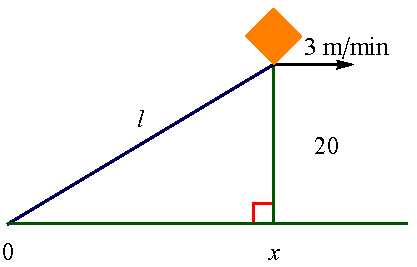
\includegraphics[width=2in]{ProductRule_fig01b}
%    \caption{Kite}
\end{figure}


\end{document}



\begin{exercise}
Suppose:
\begin{itemize}
\item $a(k)=-6$. 
\item $B(k)=-5$. 
\item $a'(k)=-9$. 
\item $B'(k)=2$. 
Comptute 
\[
\frac{d}{dk}a(k)\cdot B(k)= \answer{33}
\]
\end{exercise}

\begin{exercise}
Suppose:
\begin{itemize}
\item $F(n)=8$. 
\item $b(n)=9$. 
\item $F'(n)=8$. 
\item $b'(n)=-2$. 
Comptute 
\[
\frac{d}{dn}F(n)\cdot b(n)= \answer{56}
\]
\end{exercise}

\begin{exercise}
Suppose:
\begin{itemize}
\item $F(t)=0$. 
\item $b(t)=-6$. 
\item $F'(t)=2$. 
\item $b'(t)=7$. 
Comptute 
\[
\frac{d}{dt}F(t)\cdot b(t)= \answer{-12}
\]
\end{exercise}

\begin{exercise}
Suppose:
\begin{itemize}
\item $A(v)=-8$. 
\item $h(v)=4$. 
\item $A'(v)=7$. 
\item $h'(v)=-3$. 
Comptute 
\[
\frac{d}{dv}A(v)\cdot h(v)= \answer{52}
\]
\end{exercise}

\begin{exercise}
Suppose:
\begin{itemize}
\item $q(\theta)=2$. 
\item $G(\theta)=2$. 
\item $q'(\theta)=-5$. 
\item $G'(\theta)=8$. 
Comptute 
\[
\frac{d}{d\theta}q(\theta)\cdot G(\theta)= \answer{6}
\]
\end{exercise}

\begin{exercise}
Suppose:
\begin{itemize}
\item $q(x)=-4$. 
\item $G(x)=-10$. 
\item $q'(x)=8$. 
\item $G'(x)=-8$. 
Comptute 
\[
\frac{d}{dx}q(x)\cdot G(x)= \answer{-48}
\]
\end{exercise}

\begin{exercise}
Suppose:
\begin{itemize}
\item $r(v)=5$. 
\item $R(v)=-7$. 
\item $r'(v)=-7$. 
\item $R'(v)=-6$. 
Comptute 
\[
\frac{d}{dv}r(v)\cdot R(v)= \answer{19}
\]
\end{exercise}

\begin{exercise}
Suppose:
\begin{itemize}
\item $g(x)=-6$. 
\item $b(x)=-7$. 
\item $g'(x)=-4$. 
\item $b'(x)=-2$. 
Comptute 
\[
\frac{d}{dx}g(x)\cdot b(x)= \answer{40}
\]
\end{exercise}

\begin{exercise}
Suppose:
\begin{itemize}
\item $A(\theta)=10$. 
\item $s(\theta)=4$. 
\item $A'(\theta)=-4$. 
\item $s'(\theta)=-9$. 
Comptute 
\[
\frac{d}{d\theta}A(\theta)\cdot s(\theta)= \answer{-106}
\]
\end{exercise}

\begin{exercise}
Suppose:
\begin{itemize}
\item $P(t)=-4$. 
\item $s(t)=5$. 
\item $P'(t)=3$. 
\item $s'(t)=-7$. 
Comptute 
\[
\frac{d}{dt}P(t)\cdot s(t)= \answer{43}
\]
\end{exercise}

\begin{exercise}
Suppose:
\begin{itemize}
\item $c(\theta)=10$. 
\item $s(\theta)=10$. 
\item $c'(\theta)=7$. 
\item $s'(\theta)=6$. 
Comptute 
\[
\frac{d}{d\theta}c(\theta)\cdot s(\theta)= \answer{130}
\]
\end{exercise}

\begin{exercise}
Suppose:
\begin{itemize}
\item $F(n)=0$. 
\item $G(n)=10$. 
\item $F'(n)=3$. 
\item $G'(n)=3$. 
Comptute 
\[
\frac{d}{dn}F(n)\cdot G(n)= \answer{30}
\]
\end{exercise}

\begin{exercise}
Suppose:
\begin{itemize}
\item $P(v)=-4$. 
\item $s(v)=9$. 
\item $P'(v)=5$. 
\item $s'(v)=-4$. 
Comptute 
\[
\frac{d}{dv}P(v)\cdot s(v)= \answer{61}
\]
\end{exercise}

\begin{exercise}
Suppose:
\begin{itemize}
\item $r(n)=1$. 
\item $p(n)=-4$. 
\item $r'(n)=-5$. 
\item $p'(n)=5$. 
Comptute 
\[
\frac{d}{dn}r(n)\cdot p(n)= \answer{25}
\]
\end{exercise}

\begin{exercise}
Suppose:
\begin{itemize}
\item $r(k)=4$. 
\item $b(k)=8$. 
\item $r'(k)=-5$. 
\item $b'(k)=2$. 
Comptute 
\[
\frac{d}{dk}r(k)\cdot b(k)= \answer{-32}
\]
\end{exercise}

\begin{exercise}
Suppose:
\begin{itemize}
\item $r(u)=0$. 
\item $R(u)=-4$. 
\item $r'(u)=8$. 
\item $R'(u)=5$. 
Comptute 
\[
\frac{d}{du}r(u)\cdot R(u)= \answer{-32}
\]
\end{exercise}

\begin{exercise}
Suppose:
\begin{itemize}
\item $g(k)=5$. 
\item $p(k)=-5$. 
\item $g'(k)=3$. 
\item $p'(k)=9$. 
Comptute 
\[
\frac{d}{dk}g(k)\cdot p(k)= \answer{30}
\]
\end{exercise}

\begin{exercise}
Suppose:
\begin{itemize}
\item $r(k)=8$. 
\item $s(k)=1$. 
\item $r'(k)=5$. 
\item $s'(k)=-5$. 
Comptute 
\[
\frac{d}{dk}r(k)\cdot s(k)= \answer{-35}
\]
\end{exercise}

\begin{exercise}
Suppose:
\begin{itemize}
\item $c(w)=1$. 
\item $b(w)=2$. 
\item $c'(w)=7$. 
\item $b'(w)=8$. 
Comptute 
\[
\frac{d}{dw}c(w)\cdot b(w)= \answer{22}
\]
\end{exercise}

\begin{exercise}
Suppose:
\begin{itemize}
\item $P(\psi)=-6$. 
\item $B(\psi)=9$. 
\item $P'(\psi)=5$. 
\item $B'(\psi)=-1$. 
Comptute 
\[
\frac{d}{d\psi}P(\psi)\cdot B(\psi)= \answer{51}
\]
\end{exercise}

\begin{exercise}
Suppose:
\begin{itemize}
\item $r(x)=1$. 
\item $h(x)=2$. 
\item $r'(x)=-4$. 
\item $h'(x)=-3$. 
Comptute 
\[
\frac{d}{dx}r(x)\cdot h(x)= \answer{-11}
\]
\end{exercise}

\begin{exercise}
Suppose:
\begin{itemize}
\item $q(z)=5$. 
\item $G(z)=-8$. 
\item $q'(z)=-4$. 
\item $G'(z)=-9$. 
Comptute 
\[
\frac{d}{dz}q(z)\cdot G(z)= \answer{-13}
\]
\end{exercise}

\begin{exercise}
Suppose:
\begin{itemize}
\item $F(\psi)=4$. 
\item $h(\psi)=-5$. 
\item $F'(\psi)=-4$. 
\item $h'(\psi)=8$. 
Comptute 
\[
\frac{d}{d\psi}F(\psi)\cdot h(\psi)= \answer{52}
\]
\end{exercise}

\begin{exercise}
Suppose:
\begin{itemize}
\item $g(\psi)=5$. 
\item $h(\psi)=-10$. 
\item $g'(\psi)=6$. 
\item $h'(\psi)=5$. 
Comptute 
\[
\frac{d}{d\psi}g(\psi)\cdot h(\psi)= \answer{-35}
\]
\end{exercise}

\begin{exercise}
Suppose:
\begin{itemize}
\item $P(w)=3$. 
\item $s(w)=0$. 
\item $P'(w)=7$. 
\item $s'(w)=-2$. 
Comptute 
\[
\frac{d}{dw}P(w)\cdot s(w)= \answer{-6}
\]
\end{exercise}

\begin{exercise}
Suppose:
\begin{itemize}
\item $q(w)=-9$. 
\item $p(w)=5$. 
\item $q'(w)=0$. 
\item $p'(w)=6$. 
Comptute 
\[
\frac{d}{dw}q(w)\cdot p(w)= \answer{-54}
\]
\end{exercise}

\begin{exercise}
Suppose:
\begin{itemize}
\item $q(t)=-5$. 
\item $b(t)=-2$. 
\item $q'(t)=1$. 
\item $b'(t)=-2$. 
Comptute 
\[
\frac{d}{dt}q(t)\cdot b(t)= \answer{8}
\]
\end{exercise}

\begin{exercise}
Suppose:
\begin{itemize}
\item $F(n)=3$. 
\item $R(n)=-6$. 
\item $F'(n)=-2$. 
\item $R'(n)=-3$. 
Comptute 
\[
\frac{d}{dn}F(n)\cdot R(n)= \answer{3}
\]
\end{exercise}

\begin{exercise}
Suppose:
\begin{itemize}
\item $a(u)=3$. 
\item $s(u)=-10$. 
\item $a'(u)=3$. 
\item $s'(u)=-10$. 
Comptute 
\[
\frac{d}{du}a(u)\cdot s(u)= \answer{-60}
\]
\end{exercise}

\begin{exercise}
Suppose:
\begin{itemize}
\item $a(\theta)=-2$. 
\item $B(\theta)=8$. 
\item $a'(\theta)=-3$. 
\item $B'(\theta)=-7$. 
Comptute 
\[
\frac{d}{d\theta}a(\theta)\cdot B(\theta)= \answer{-10}
\]
\end{exercise}

\begin{exercise}
Suppose:
\begin{itemize}
\item $F(x)=-4$. 
\item $R(x)=0$. 
\item $F'(x)=8$. 
\item $R'(x)=4$. 
Comptute 
\[
\frac{d}{dx}F(x)\cdot R(x)= \answer{-16}
\]
\end{exercise}

\begin{exercise}
Suppose:
\begin{itemize}
\item $g(w)=8$. 
\item $R(w)=6$. 
\item $g'(w)=4$. 
\item $R'(w)=4$. 
Comptute 
\[
\frac{d}{dw}g(w)\cdot R(w)= \answer{56}
\]
\end{exercise}

\begin{exercise}
Suppose:
\begin{itemize}
\item $g(w)=-10$. 
\item $p(w)=-5$. 
\item $g'(w)=-9$. 
\item $p'(w)=-6$. 
Comptute 
\[
\frac{d}{dw}g(w)\cdot p(w)= \answer{105}
\]
\end{exercise}

\begin{exercise}
Suppose:
\begin{itemize}
\item $g(v)=4$. 
\item $h(v)=-6$. 
\item $g'(v)=3$. 
\item $h'(v)=-10$. 
Comptute 
\[
\frac{d}{dv}g(v)\cdot h(v)= \answer{-58}
\]
\end{exercise}

\begin{exercise}
Suppose:
\begin{itemize}
\item $a(n)=-9$. 
\item $b(n)=4$. 
\item $a'(n)=1$. 
\item $b'(n)=-1$. 
Comptute 
\[
\frac{d}{dn}a(n)\cdot b(n)= \answer{13}
\]
\end{exercise}

\begin{exercise}
Suppose:
\begin{itemize}
\item $F(x)=-2$. 
\item $h(x)=-6$. 
\item $F'(x)=-9$. 
\item $h'(x)=-9$. 
Comptute 
\[
\frac{d}{dx}F(x)\cdot h(x)= \answer{72}
\]
\end{exercise}

\begin{exercise}
Suppose:
\begin{itemize}
\item $A(w)=3$. 
\item $G(w)=4$. 
\item $A'(w)=-1$. 
\item $G'(w)=-1$. 
Comptute 
\[
\frac{d}{dw}A(w)\cdot G(w)= \answer{-7}
\]
\end{exercise}

\begin{exercise}
Suppose:
\begin{itemize}
\item $r(v)=9$. 
\item $R(v)=-10$. 
\item $r'(v)=8$. 
\item $R'(v)=-5$. 
Comptute 
\[
\frac{d}{dv}r(v)\cdot R(v)= \answer{-125}
\]
\end{exercise}

%\end{shuffle}

\end{document}
